\documentclass[11pt]{article}

\usepackage{float}
\usepackage{hyperref}
\usepackage{graphicx}
% formatting
\usepackage{fullpage}
\usepackage{verbatim}
\usepackage{moreverb}
\usepackage{minted}
\usepackage{parskip}
\usepackage{amsmath}
\let\verbatiminput=\verbatimtabinput
\def\verbatimtabsize{4\relax}

\begin{document}
\title{EECS 151/251A FPGA Lab\\
Lab 2: Simulation, Inter-module Communication, and Memories}

\author{Prof. Elad Alon \\
TAs: Vighnesh Iyer, Bob Zhou \\Department of Electrical Engineering and Computer Sciences\\
College of Engineering, University of California, Berkeley}
\date{}
\maketitle

\tableofcontents

\section{Before You Start This Lab}

Before you proceed with the contents of this lab, we suggest that you look through three documents that will help you better understand some Verilog constructs.

\begin{enumerate}
	\item \textbf{labs\_sp17/docs/Verilog/wire\_vs\_reg.pdf} - The differences between wire and reg nets and when to use each of them.
	
	\item \textbf{labs\_sp17/docs/Verilog/always\_at\_blocks.pdf} - Understanding the differences between the two types of always @ blocks and what they synthesize to.
	
	\item \textbf{labs\_sp17/docs/Verilog/verilog\_fsm.pdf} - An overview of how to create finite state machines in Verilog, specifying their state transitions and machine outputs.
\end{enumerate}

The first couple sections of this lab focus on simulation and it would be valuable to read the first two documents before starting.

\subsection{Helpful Hint: Synthesis Warnings and Errors}
At various times in this lab, things will just not work on the FPGA or in simulation. To help with debugging, you can run \verb|make synth| in the \verb|lab2/| folder. This will just run \verb|xst| (Synthesis) which will only take a few seconds. Then you should run \verb|make report|. In the window that opened, click on \verb|Synthesis Messages| on the left under \verb|Errors and Warnings|. Any synthesis warnings you see here are an alert to a possible issue in your circuit. If you don't understand a warning, ask a TA; it could reveal some issue in your Verilog.

\section{Lab Overview}

In this lab, we will begin by taking your \verb|tone_generator| design from Lab 1 and simulating it in software. We will learn how to use ModelSim to view waveforms and debug your circuits. You will then extend your \verb|tone_generator| to play a configurable frequency square wave and simulate it to check that you have implemented the functionality correctly. You will then construct a module that can pull tones to play from a memory block and send them to your \verb|tone_generator|.

\section{Simulating the tone\_generator from Lab 1}

\subsection{Copying Your Lab 1 Code}

Run \verb|git pull| in your git cloned \verb|labs_sp17| directory to fetch the latest skeleton files.

Begin by copying your \verb|tone_generator| implementation into the \verb|lab2/src/tone_generator.v| file. \textbf{Don't change the module port declaration.} You can leave the \verb|input [23:0] tone_switch_period| unused for now.

Let's run some simulations on the \verb|tone_generator| in software. To do this, we will need to use a Verilog testbench. A Verilog testbench is designed to test a Verilog module by supplying it with the inputs it needs (stimulus signals) and testing whether the outputs of the module match what we expect.

\subsection{Overview of Testbench Skeleton}
Check the provided testbench skeleton in \verb|lab2/tone_generator_testbench.v| to see the test written for the \verb|tone_generator|. Let's go through what every line of this testbench does.

\begin{minted}{verilog}
`timescale 1ns/1ns
`timescale (simulation step time)/(simulation resolution)
\end{minted}

The timescale declaration needs to be at the top of every testbench file. It provides information to the circuit simulator about the timing parameters of the simulation.

The first argument to the timescale declaration is the simulation step time. It defines the chunks of discrete time in which the simulation should proceed. In this case, we have defined the simulation step time to be one nanosecond. This means that we can advance the simulation time by as little as 1ns at a time.

The second argument to the timescale declaration is the simulation resolution. In our example it is also 1ns. The resolution allows the simulator to model transient behavior of your circuit in between simulation time steps. For this lab, we aren't modeling any gate delays, so the resolution can equal the step time.

\begin{minted}{verilog}
`define SECOND 1000000000
`define MS 1000000
// The SAMPLE_PERIOD corresponds to a 44.1 kHz sampling rate
`define SAMPLE_PERIOD 22675.7
\end{minted}

These are some macros defined for our testbench. They are constant values you can use when writing your testbench to simplify your code and make it obvious what certain numbers mean. For example, \verb|SECOND| is defined as the number of nanoseconds in one second. The \verb|SAMPLE_PERIOD| is the sampling period used to sample the square wave output of the \verb|tone_generator| at a standard 44.1 kHz sample rate.

\begin{minted}[tabsize=4]{verilog}
module tone_generator_testbench();
	// Testbench code goes here
endmodule
\end{minted}

This module is our testbench module. It is not actually synthesized to be placed on our FPGA, but rather it is to be run by our circuit simulator. All your testbench code goes in this module. We will instantiate our DUT (device under test) in this module.

\begin{minted}{verilog}
reg clock;
reg output_enable;
reg [23:0] tone_to_play;
wire sq_wave;
\end{minted}

Here are the inputs and outputs of our \verb|tone_generator|. You will notice that the inputs to the \verb|tone_generator| are declared as \verb|reg| type nets and the outputs are declared as \verb|wire| type nets. This is because we will be driving the inputs in our testbench and we will be monitoring the output.

\begin{minted}{verilog}
initial clock = 0;
always #(30.3/2) clock <= ~clock;
\end{minted}

Here is our clock signal generation code. The clock signal needs to be generated in our testbench so it can be fed to the DUT. The initial statement sets the value of the clock net to 0 at the very start of the simulation. The next line toggles the clock signal such that it oscillates at 33Mhz.

\begin{minted}[tabsize=4]{verilog}
tone_generator piezo_controller (
    .clk(clock),
    .output_enable(output_enable),
	.tone_switch_period(tone_to_play),
    .square_wave_out(sq_wave)
);
\end{minted}

Now we instantiate the DUT and connect its ports to the nets we have access to in our testbench.

\begin{minted}[tabsize=4]{verilog}
initial begin
    output_enable <= 0;
    #(10 * `MS);
    output_enable <= 1;
    
    tone_to_play <= 24'd37500;
    #(200 * `MS);
   
    ...
    $finish();
end
\end{minted}

Here is the body of our testbench. The \verb|initial begin ... end| block specifies the 'main()' function for our testbench. It is the execution entry point for our simulator. In the \verb|initial| block, we can set the inputs that flow into our DUT using non-blocking (\verb|<=|) assignments.

We can also order the simulator to advance simulation time using delay statements. A delay statement takes the form \verb|#(delay in time steps);|. For instance the statement \verb|#(100);| would run the simulation for 100ns.

In this case, we set \verb|output_enable| to 0 at the start of the simulation, then we let the simulation run for 10ms, then we set \verb|output_enable| to 1. We then change the \verb|tone_to_play| several times, and give the \verb|tone_generator| some time to produce the various tones. For now, the \verb|tone_to_play| signal won't affect your \verb|tone_generator| which should only be playing a fixed 440 Hz tone.

The final statement is a system function: the \verb|$finish()| function tells the simulator to halt the simulation.

\begin{minted}[tabsize=4]{verilog}
integer file;
initial begin
	file = $fopen("output.txt", "w");
	forever begin
		$fwrite(file, "%h\n", sq_wave);
		#(`SAMPLE_PERIOD);
	end
end
\end{minted}

This piece of code is written in a separate \verb|initial begin ... end| block. The simulator treats both blocks as separate threads that both start execution at the beginning of the simulation and operate in parallel.

This block of code uses two system functions \verb|$fopen() and $fwrite()|, that allow us to write to a file. The \verb|forever begin| construct tells the simulator to run the chunk of code inside it continuously until the simulation ends.

In the \verb|forever begin| block, we sample the \verb|square_wave_out| output of the \verb|tone_generator| and save it in a file. We sample this value every \verb|`SAMPLE_PERIOD| nanoseconds which corresponds to a 44100 kHz sampling rate. Your \verb|tone_generator|'s output is stored as 1s and 0s in a text file that can be translated to sound to hear how your circuit will sound when deployed on the FPGA.

\subsection{Using TCL scripts (.do files)}

\textbf{ModelSim}, which is our circuit simulator, takes commands from TCL scripts. Take a look at the \verb|lab2/sim/tests/tone_generator_testbench.do| TCL script. Here is a quick description of what is instructs our simulator to do.

\begin{minted}{tcl}
start tone_generator_testbench
add wave tone_generator_testbench/*
add wave tone_generator_testbench/piezo_controller/*
run 10000ms
\end{minted}

We begin by issuing the \verb|start| command to the simulator. This instructs the simulator to scan a list of Verilog source files provided to it to find a module named \verb|tone_generator_testbench|. This module name must exactly match the module name of your top-level testbench module. The simulator loads and elaborates this module so that its ready to simulate/execute.

The two \verb|add_wave| commands are important. By default, the simulator will not log the signals in our testbench or DUT as the simulation executes. The \verb|add wave tone_generator_testbench/*| line tells the simulator to log all signals directly inside in the \verb|tone_generator_testbench| module. The second line tells the simulator to log the signals in a submodule of the top-level testbench module. Observe that \verb|piezo_controller| is the instance name of the \verb|tone_generator| instance in the testbench module.

Finally, the \verb|run (time)| command tells the simulator to jump to the \verb|initial begin| blocks in the testbench and actually run the simulation. The time value (in our case 10000ms = 10s) gives the simulator an upper bound on the simulation time. The simulator will simulate for 10 seconds before timing out. If the simulator hits the \verb|$finish()| function before the 10 second timeout is up, it will stop simulation instantly.

\subsection{Running ModelSim}

With all the details out of the way, let's actually run a simulation. Go to the \verb|lab2/sim| directory and run \verb|make|. After a minute or so, the simulation will finish.

\subsection{Viewing Waveforms}

Let's take a look at the data that the simulator collected. Run the viewwave script like this:

\verb|./viewwave results/tone_generator_testbench.wlf &|

The results of the simulation and the logged signals are stored in a \verb|.wlf| file. This command should open that file in the ModelSim Wave Viewer.

You should see a window like this:

\begin{figure}[H]
	\centerline{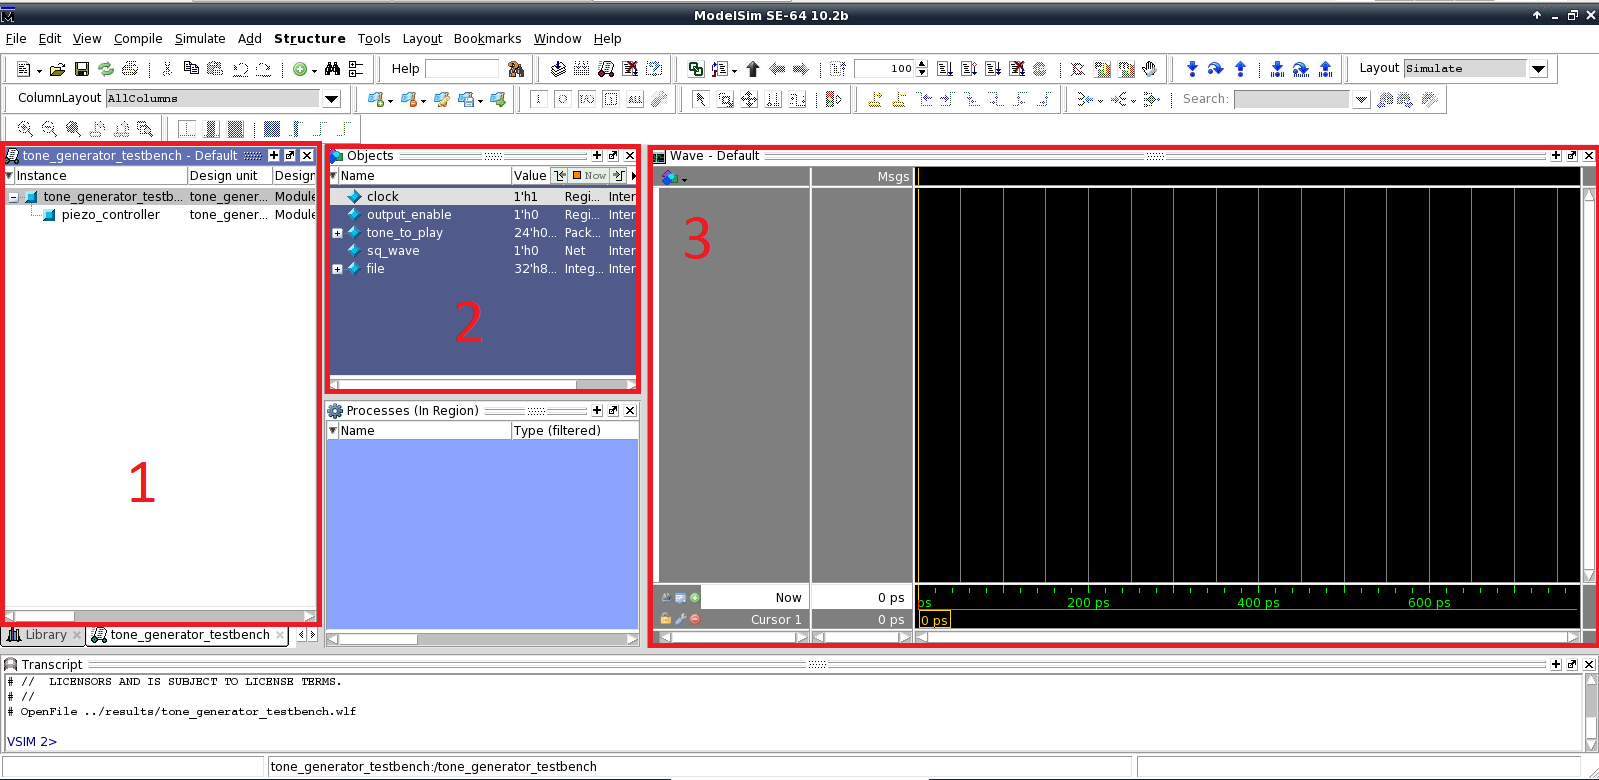
\includegraphics[width=\textwidth]{images/modelsim_new.png}}
\end{figure}

Let's go over the basics of ModelSim. The boxed screens are:

\begin{enumerate}
	\item \textbf{Module Window} - List of the modules involved in the testbench. You can select one of these to have its signals show up in the object window.
	\item \textbf{Object Window} - List of all the wires and regs in the selected module. You can add signals to the waveform view by selecting them, right-clicking, and doing \verb|Add Wave|.
	\item \textbf{Waveform Viewer} - The signals that you add from the object window show up here. You can navigate the waves by searching for specific values or going forward or backward one transition at a time. The x-axis represents time.
\end{enumerate}

You may not see the \textbf{Waveform Viewer} when you first open ModelSim. To add signals to view, right click on the signal in the \textbf{Object Window}, and click on \verb|Add Wave|. Add the \verb|clock, output_enable,| and \verb|sq_wave| signals to the waveform viewer.

Here are a few useful shortcuts:

\begin{itemize}
	\item \textbf{Click on waveform}: Sets cursor position
	\item \textbf{O}: Zoom out of waveform
	\item \textbf{I}: Zoom into waveform
	\item \textbf{F}: Fit entire waveform into viewer (zoom full)
	\item \textbf{C}: Zoom in on cursor position
	\item \textbf{Middle Click + Drag Left/Right}: Zoom in on waveform section
	\item \textbf{Middle Click + Drag to Top Right}: Zoom out from current waveform section
\end{itemize}

You should play with these shortcuts for a few minutes; they will boost your productivity when debugging greatly. Now, zoom to fit the entire waveform in your viewer.

You should be able to see the clock oscillate at the frequency specified in the testbench. You should also see the \verb|output_enable| signal start at 0 and then become 1 after 10 ms. However, you may see that the \verb|sq_wave| signal is just a red line. What's going on?

\subsection{Fixing the Undefined clock\_counter}

Take a look at the \verb|clock_counter|, by clicking on \verb|piezo_controller| in the module and \verb|Add Wave| on the \verb|clock_counter| signal. Plot the signal in your waveform viewer. You may notice it's a red line. Red lines in ModelSim indicate undefined signals (defined in Verilog as the letter \verb|x|).

Blue lines in ModelSim indicate high-impedance (unconnected) signals. High-impedance is defined in Verilog as the letter \verb|z|. We won't be using high-impedance signals in our designs, so blue lines in ModelSim indicate something in our testbench isn't wired up properly.

Going back to the red line for \verb|clock_counter|: this is caused because at the start of simulation, the value sitting inside the \verb|clock_counter| register is unknown. It could be anything! Since we don't have an explicit reset signal for our circuit to bring the \verb|clock_counter| to a defined value, it may be unknown for the entire simulation.

Let's fix this. In the future we will use a reset signal, but for now let's use a simpler technique. In \verb|lab2/src/tone_generator.v| modify this line as such:

\begin{minted}{verilog}
// Original code:
reg [x:0] clock_counter;

// Change to:
reg [x:0] clock_counter = 0;
\end{minted}

This tells the simulator that the initial simulation value for this register should be 0. For this lab, when you add new registers in your \verb|tone_generator| or any other design module, you should instantiate them to their initial value in the same way. \textbf{Do not set an initial value for a 'wire' type net; it will cause issues with synthesis, and may cause X's in simulation.}

Now run the simulation again.

\subsubsection{Helpful Tip: Reloading ModelSim .wlf}

When you re-run your simulation and you want to plot the newly generated signals in ModelSim, you don't need to close and reopen ModelSim. Instead click on the 'Reload' button on the top toolbar which is to the right of the 'Save' button.

\subsection{Listen to Your Square Wave Output}

Take a look at the file written by the testbench located at \verb|lab2/sim/build/output.txt|. It should be a sequence of 1s and 0s that represent the output of your \verb|tone_generator| sampled at 44.1 kHz. I've written a Python script that can take this file and generate a \verb|.wav| file that you can listen to.

Go to the \verb|lab2/| directory and run the command:

\verb|python scripts/audio_from_sim.py sim/build/output.txt|

This will generate a file called \verb|output.wav|. Run this command to play it:

\verb|play output.wav|

If \verb|play| doesn't work, try running \verb|aplay output.wav|.

You should hear a 440Hz square wave for 1 second.

\subsection{Playing with the Testbench}

Play around with the testbench by altering the clock frequency, changing when you turn on \verb|output_enable| and verify that you get the audio you expect. For checkoff be able to answer the following question and demonstrate understanding of basic simulation:

\begin{enumerate}
	\item If you increase the clock frequency from 33 Mhz, would you expect the tone generated by your \verb|tone_generator| to be of a higher or lower frequency than 440Hz? Why? Show audio evidence of this using simulation.
	\item Prove that the \verb|output_enable| input of your \verb|tone_generator| actually works in simulation.
\end{enumerate}

\section{Design a Configurable Frequency tone\_generator}

Let's extend our \verb|tone_generator| so that it can play different notes. Notice that we have a 24-bit input to the \verb|tone_generator| called \verb|tone_switch_period|. Note you will also have to modify your \verb|clock_counter| to be 24 bits wide.

The \verb|tone_switch_period| describes how often the square wave output switches from high to low or low to high. For example a \verb|tone_switch_period| of 37500 tells us to invert the square wave output every 37500 clock cycles, which for a 33 Mhz clock translates to a 440 Hz square wave. Here is the derivation for review:

\begin{eqnarray}
	\frac{33 \times 10^6 \text{ cycles}}{1 \text{ second}} \div \frac{440 \text{ periods}}{1 \text{ second}} = \frac{75000 \text{ cycles}}{1 \text{ period}} \nonumber \\
	75000 \text{ cycles/period} \rightarrow 37500 \text{ cycles/half-period} \nonumber
\end{eqnarray}

You may have to modify the architecture of your \verb|tone_generator| to accommodate this new input signal. You should reset the internal \verb|clock_counter| every \verb|tone_switch_period| cycles and should also invert the square wave output. Remember to initialize any new registers declared in your \verb|tone_generator| to their desired initial value to prevent unknowns during simulation.

\section{Simulating and Debugging Your New tone\_generator}

Now, let's run the \verb|tone_generator_testbench| again. Since we have now implemented the \verb|tone_switch_period| functionality, changing the \verb|tone_to_play| register in the testbench should change the tone being outputted by the \verb|tone_generator|.

Inspect the waveform and debug your \verb|tone_generator| if you detect any bugs. Then use the same Python script to generate an audio file to listen to your \verb|tone_generator|'s output. You should hear 5 tones, played rapidly one after the other that have descending frequencies.

Create a testbench that plays some simple melody that you define and have its audio output file ready for checkoff.

\section{Try the tone\_generator on the FPGA}
Modify the top-level Verilog module \verb|ml505top.v| to include the new input to the \verb|tone_generator|. You should tie the \verb|tone_switch_period| to the \verb|GPIO_DIP[7:1]| switches left-shifted by 9 bits (effectively a multiplication by 512). This will allow you to control the \verb|tone_switch_period| from 512 to around 65000. Leave \verb|GPIO_DIP[0]| to control \verb|output_enable|. Here is a code snippet:

\begin{minted}[tabsize=4]{verilog}
	tone_generator piezo_controller (
		.output_enable(GPIO_DIP[0]),
		.tone_switch_period({17'd0, GPIO_DIP[7:1]} << 9)
	);
\end{minted}

Run the usual \verb|make| process and then \verb|make impact| to put your new \verb|tone_generator| on the FPGA. Verify that toggling the DIP switches changes the frequency of your \verb|tone_generator|. 

\section{Introduction to Inferred Asynchronous Memories - ROMs}
An asynchronous memory is a memory block that isn't governed by a clock. In this lab, we will use a Python script to generate a ROM block in Verilog.

A ROM is a read-only memory. A ROM can be broadly classed as a state element that holds some fixed data. This data can be accessed by supplying an address to the ROM; after some time, the ROM will output the data stored at that address. A memory block in general can contain as many addresses in which to store data as you desire. Every address should contain the same amount of data (bits). The number of addresses is called the \textbf{depth} of the memory, while the number of bits stored per address is called the \textbf{width} of the memory. These are important terms that are frequently used.

The synthesizer is a powerful tool that takes the Verilog you write and converts it into a low-level netlist of the structures are actually used on the FPGA. Our Verilog \textbf{describes} the functionality of some digital circuit and the synthesizer \textbf{infers} what primitives implement the functional description. In this section, we will examine the Verilog that allows the synthesizer (XST) to \textbf{infer} a ROM. What follows is a minimal example of a ROM in Verilog: (depth of 8 entries/addresses, width of 12 bits)

\begin{minted}[tabsize=4]{verilog}
module rom (input [2:0] address, output reg [11:0] data);
	always @(*) begin
		case(address)
			3'd0: data = 12'h000;
			3'd1: data = 12'hFFF;
			3'd2: data = 12'hACD;
			3'd3: data = 12'h122;
			3'd4: data = 12'h347;
			3'd5: data = 12'h93A;
			3'd6: data = 12'h0AF;
			3'd7: data = 12'hC2B;
		endcase
	end
endmodule
\end{minted}

To power our \verb|tone_generator|, we will be using a ROM that is X entries/addresses deep and 24 bits wide. The ROM will contain tones that the \verb|tone_generator| will play. You can choose the depth of your ROM based on the length of the sequence of tones you want to play.

We've provided you with a few scripts that can generate a ROM from either a file with it's contents or even from sheet music. Run these commands from \verb|lab2/|.

\begin{minted}{bash}
python scripts/musicxml_parser.py musicxml/Twinkle_Twinkle_Little_Star.mxl music.txt
python scripts/rom_generator.py music.txt src/rom.v 1024 24
\end{minted}

The first script will parse a MusicXML file and turn it into a list of \verb|tone_switch_periods| for each of the notes for a piece of sheet music. The second script will take that list and turn it into a ROM that's 1024 entries deep with a width of 24 bits.

Take a look at \verb|music.txt| and \verb|src/rom.v|. You can download your own music in MusicXML format from here (\url{https://musescore.org/}) and run it through the same parser; it should ideally only have one part to work properly. You can also directly edit the \verb|music.txt| file to customize the contents of the ROM as you wish.

\section{Design of the music\_streamer}
Open up the \verb|music_streamer.v| file. This module will contain an instance of the ROM you created earlier and will address the ROM sequentially to play notes. The \verb|music_streamer| will play each note in the ROM for a predefined amount of time by sending it to the \verb|tone_generator|. 

We will play each note for 1/25th of a second. Calculate what that is in terms of 33Mhz clock cycles.

Begin by instantiating the \verb|music_streamer| module in \verb|ml505top.v|. Use the instance name \verb|streamer| to match the expected name in the \verb|.do| file. Connect its \verb|tone| output to the \verb|tone_switch_period| input of the \verb|tone_generator|. Connect its \verb|clk| input to the global clock signal. Connect its \verb|rom_address| output to the \verb|GPIO_LED|s by routing the top 8 bits of the address to the LEDs.

Now let's begin the design of the \verb|music_streamer| itself. Instantiate your ROM in the \verb|music_streamer| and connect the ROM's \verb|address| and \verb|data| ports to wire or reg nets that you create in your module (you can ignore the \verb|last_address| port).

Next, write the RTL that will increment the address supplied to the ROM every \textbf{1/25th of a second}. The data coming out of the ROM should be fed directly to the \verb|tone| output. The ROM's address input should go from 0 to the depth of the ROM and should then loop around back to 0. You don't have a reset signal, so define the initial state of any registers in your design for simulation purposes. Also hook up the \verb|rom_address| output to the ROM address currently being accessed.

\section{Simulating the music\_streamer}
To simulate your \verb|music_streamer| open up the \verb|lab2/src/music_streamer_testbench.v|. In contrast to the \verb|tone_generator_testbench| where the \verb|tone_generator| was instantiated in isolation, in this testbench we are instantiating our entire top-level design, \verb|ml505top|. This testbench is referred to as a system-level testbench, which tests our entire design using top-level I/O, in contrast to the \verb|tone_generator_testbench| which is a block-level testbench. This is similar to the difference between unit and integration tests in software development.

You can see that this testbench just runs a simulation for 2 seconds and then exits. To run this simulation, go to \verb|lab2/sim/tests| and change the extension on the \verb|music_streamer_testbench.dont| file to \verb|.do|. Our Makefile works by executing the TCL files in this folder that have the file extension \verb|.do|. You might have to modify the \verb|.do| file to match the name of your module instances in \verb|ml505top.v|.

To execute the testbench, run \verb|make| in \verb|lab2/sim|. This may take several minutes to complete. You may have to run \verb|make clean| before running \verb|make| if ModelSim has cached build artifacts.

Inspect your waveform to make sure you get what you expect. Verify that there are no undefined signals (red lines, x) Then, run the Python script to generate a \verb|.wav| file of your simulation results and listen to your \verb|music_streamer| in action. It should sound like the first few seconds of the song that was loaded on the ROM.

\section{Verify your Code to Works For Rest Notes}
In simulation, you can often catch bugs that would be difficult or impossible to catch by running your circuit on the FPGA. You should verify that if your ROM contains an entry that is zero (i.e. generate a 0Hz wave), that the \verb|tone_generator| holds the \verb|square_wave_out| output at either 1 or 0 with no oscillation. Verify this in simulation, and prove the correct functionality during checkoff.

\section{Try it on the FPGA!}
Now try your \verb|music_streamer| on the FPGA. You should expect the output to be the same as in simulation. The \verb|GPIO_DIP[0]| switch should still work to disable the output of the \verb|tone_generator|. \textbf{Show your final results, simulation, and the working design on the FPGA to the TA for checkoff.}

\section{Optional: Adding Tempo Variations and Pausing to the music\_streamer}
In the next lab, we will be making our \verb|music_streamer| more full-featured. If you have time now, you can implement some of these features.

Connect a \verb|GPIO_DIP| switch to a new \verb|pause| input of the \verb|music_streamer|. When this switch is turned on, your module should pause the music at the current note and should cut the output to the piezo speaker. When the switch is turned off, your module should resume playback.

Connect a pair of \verb|GPIO_DIP| switches to a new \verb|tempo| input of the \verb|music_streamer|. When these switches are toggled, your \verb|music_streamer| should play the notes faster or slower. Basically, you can define four different tempos that hold each note for a different amount of time. We choose a standard 1/25th of a second for this lab, but you can vary it from 1/75, 1/50, 1/30, 1/15 to change the tempo of your music playback on the fly.

\section{Checkoff}
\begin{enumerate}
	\item Section 3.8 - How will a higher clock frequency impact the frequency of the square wave output for a fixed \verb|tone_switch_period|?
	\item Section 5 - Play an audio file that was generated using the \verb|tone_generator_testbench| that plays some melody you define.
	\item Section 10 - Prove that if the ROM contains an entry for a \verb|tone_switch_period| of 0, that the square wave doesn't oscillate.
	\item Section 11 - Show the working \verb|music_streamer| on the FPGA.
\end{enumerate}

\section{Conclusion}
You are done with lab 2! Please write down any and all feedback and criticism of this lab and share it with the TA. This is a new lab and we welcome everyone's input so that it can be improved.

\end{document}